Pour faciliter la compréhension d'un problème, nous avons tendance à le dessiner ce qui nous amène parfois même à le résoudre. La théorie des graphes est fondée à l'origine sur ce principe. De nombreuses propriétés et méthodes ont été pensées ou trouvées à partir d'une représentation schématique pour être ensuite formalisées et prouvées.


La théorie des graphes est historiquement un domaine mathématique qui s'est développé  au sein d'autres disciplines comme la chimie, la biologie, la sociologie et l'industrie. Elle constitue aujourd'hui un corpus de connaissances très important et un instrument efficace pour résoudre une multitude de problèmes.


De manière générale, le graphe sert à représenter les structures, les connexions entre différents composants, les acheminements possibles pour un ensemble complexe composé d'un grand nombre de situations en exprimant les dépendances et les relations entre ses éléments,(e.g. réseau routier ou ferroviaire, réseau de communication, diagramme d'ordonnancement, ..). 


Dans ce chapitre, nous présenterons les notions et les concepts clés relatifs aux graphes qui serviront de base pour la suite de notre travail, à savoir : la définition d'un graphe, ses types et sa représentation structurelle. Nous clôturons le chapitre avec quelques domaines d'application des graphes.

	
	\section{Graphe non orienté}
			\subsection{Définitions et généralités}
		
Un graphe non orienté G est la donnée d’un couple (V , E) où V = \{$ \textit{v}_{1} , \textit{v}_{2} ,..., \textit{v}_{n} $\} est un ensemble fini dont les éléments sont appelés sommets ou nœuds ( Vertices en anglais ) et  E=\{$\textit{e}_{1} ,  \textit{e}_{2} ,…, \textit{e}_{m} $\} est un ensemble fini d'arêtes ( Edges en anglais ). Toute arête \textit{e} de E correspond à un couple non ordonné de sommets ( $\textit{v}_{i} , \textit{v}_{j}$ ) $\in$ E $\subset$  $V \times V$ représentant ses extrémités \citep{muller} \citep{fages2014exploitation}.
\\Soient \textit{e} = ($\textit{v}_{i} , \textit{v}_{j}$) et \textit{e'}=($\textit{v}_{k} , \textit{v}_{l}$) deux arêtes de E, On dit que :
\begin{itemize}
\item $\textit{v}_{i}$ et $\textit{v}_{j}$ sont les extrémités de \textit{e} et \textit{e} est incidente à $\textit{v}_{i}$ et $\textit{v}_{j}$ \citep{hennecart2012elements}.
\item $\textit{v}_{i}$ et $\textit{v}_{j}$ sont voisins ou adjacents, s'il y a au moins une arête entre eux dans E \citep{IUTLyonInformatique}.
\item L'ensemble des sommets adjacents aux deux extrémités de \textit{e} est appelé le voisinage de \textit{e} \citep{muller}. 
\item \textit{e} et \textit{e'} sont voisins s'ils ont une extrémité commune  \citep{lopez2003cours}.
\item L'arête \textit{e} est une boucle si ses extrémités coïncident, i.e, $\textit{v}_{i}$ = $\textit{v}_{j}$ \citep{IUTLyonInformatique}. 
\item L'arête \textit{e} est multiple si elle a plus d'une seule occurrence dans l'ensemble E.
\end{itemize}	
		 
\subsection{Représentation graphique}
Un graphe non orienté G peut être représenté par un dessin sur un plan comme suit \citep{muller}:

\begin{itemize}
\item Les nœuds $\textit{v}_{i}$ $\in$ V de G sont représentés par des points distincts.
\item 	Les arêtes \textit{e} = ($\textit{v}_{i}$,$\textit{v}_{j}$) $\in$ E de G sont représentés par des lignes, pas forcement rectilignes, qui relient les extrémités de chaque arête \textit{e}.
\end{itemize}

%% L'exemple de la représentation graphique 
\textbf{Exemple :}
 Soit g=(V1 , E1) un graphe non orienté tel que : V1=\{ 1,2,3,4,5 \} et E1=\{(1,2), (1,4), (2,2), (2,3), (2,5), (3,4)\}.
La représentation graphique de g est alors donnée par le schéma de la figure \ref{graphNonOriente}.
\\
\begin{figure}[H]
\begin{center}
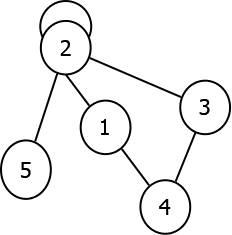
\includegraphics[height=120 pt, width=130 pt]{./ressources/image/graphNonOriente.png} 
\end{center}
\caption{Exemple de représentation graphique d'un graphe non orienté}
\label{graphNonOriente}
\end{figure}

		\subsection{Propriétés d'un graphe}
		
		\begin{itemize}[label=$\circ$]
			
			\item \textbf{Ordre d'un graphe:} On appelle ordre d’un 					graphe le nombre de ses sommets, i.e, Card(V) \citep{DUT}.
			
			\item  \textbf{Taille d'un graphe:} On appelle taille d’un 				graphe le nombre de ses arêtes, i.e, Card(E) \citep{DUT}.
			
			\item  \textbf{Degré dans un graphe:}
			
			
			\begin{itemize}[label=$\bullet$]
				\item \textbf{Degré d'un sommet : } Le degré d’un sommet noté \textit{d}($\textit{v}_{i}$) est le nombre d'arêtes incidentes à ce sommet, sachant qu’une boucle compte pour deux \citep{muller}. Dans l'exemple de la figure \ref{graphNonOriente}, le degré du sommet (1) est : \textit{d}(1)=2.
				
				\item \textbf{Degré d'un graphe : }Le degré d’un graphe est le degré maximum de ses sommets, i.e, max(\textit{d}($\textit{v}_{i}$)) \citep{muller}. Dans l’exemple de 				la figure \ref{graphNonOriente}, le degré du graphe g est \textit{d}(2)=5.
			\end{itemize}
			
			\item \textbf{Rayon et diamètre dans un graphe:}
			\begin{itemize}[label=$\bullet$]
				\item \textbf{Distance : }La distance entre deux sommets 	\textit{v} et \textit{u} est le plus petit nombre d’arêtes qu’on doit parcourir pour aller de \textit{v} à \textit{u} ou de \textit{u} à \textit{v} \citep{muller}. 
				
				\item 	\textbf{Diamètre d’un graphe :} C’est la plus grande 	distance entre deux sommets de ce graphe \citep{muller}. 
				
				\item 	\textbf{Rayon d’un graphe : }C’est la plus petite distance entre deux sommets de ce graphe \citep{parlebas1972centralite}. 
			\end{itemize}
		\end{itemize}
		
	
			
	
			
	\section{Graphe orienté}	
		
		\subsection{Définitions et généralités}
		Un graphe orienté G est la donnée d'un couple (V , E) où
		V est un ensemble fini dont les éléments sont appelés les sommets de G et 
		E  $\subset$ V x V est un ensemble de couples ordonnés de sommets dits arcs ou arêtes \citep{muller}. G est appelé dans ce cas digraphe (directed graph).\\
		 Pour tout arc e = ( $v_{i}$ , $v_{j}$) $\in$ E :
		 \begin{itemize}  
			\item $v_{i}$ est dit extrémité initiale ou origine de e et $v_{j}$ est l'extrémité finale de e \citep{muller}.
			
			\item $v_{i}$ est le prédécesseur de $v_{j}$ et $v_{j}$ est le successeur de $v_{i}$ \citep{IUTLyonInformatique}.
			
			\item les sommets $v_{i}$ , $v_{j}$ sont des sommets adjacents \citep{Pres}.
			
			\item e est dit sortant en $v_{i}$ et incident en $v_{j}$ \citep{Pres}.
			
			\item e est appelé boucle si $v_{i}$ = $v_{j}$, i.e l'extrémité initiale et finale représente le même sommet \citep{IUTLyonInformatique}.
			
		\end{itemize}
		 
		
		\subsection{Représentation graphique}
		
		
		Un graphe G = (V , E) peut être projeter sur le plan en représentant:
		\begin{itemize} 
		\item Dans un premier temps les nœuds $v_{i}$ $\in$ V par des points disjoints du plan.
		\item Et dans un second temps les arêtes e = ( $v_{i}$ , $v_{j}$) $\in$ E par des lignes orientées reliant par des flèches les deux extrémités de e. 
		\end{itemize}
		
		\textbf{Exemple:}
		
		Soit g = ($V_{1}$ , $E_{1}$) un digraphe tel que : $V_{1}$ = \{ 1,2,3,4 \} et  $E_{1}$ = \{(1,2),(1,3),(3,2),(3,4),(4,3)\}.
		
		Le représentation graphique de g est alors donné par le schéma de la figure \ref{grapheOr}.
	
		
			\begin{figure}[h]
			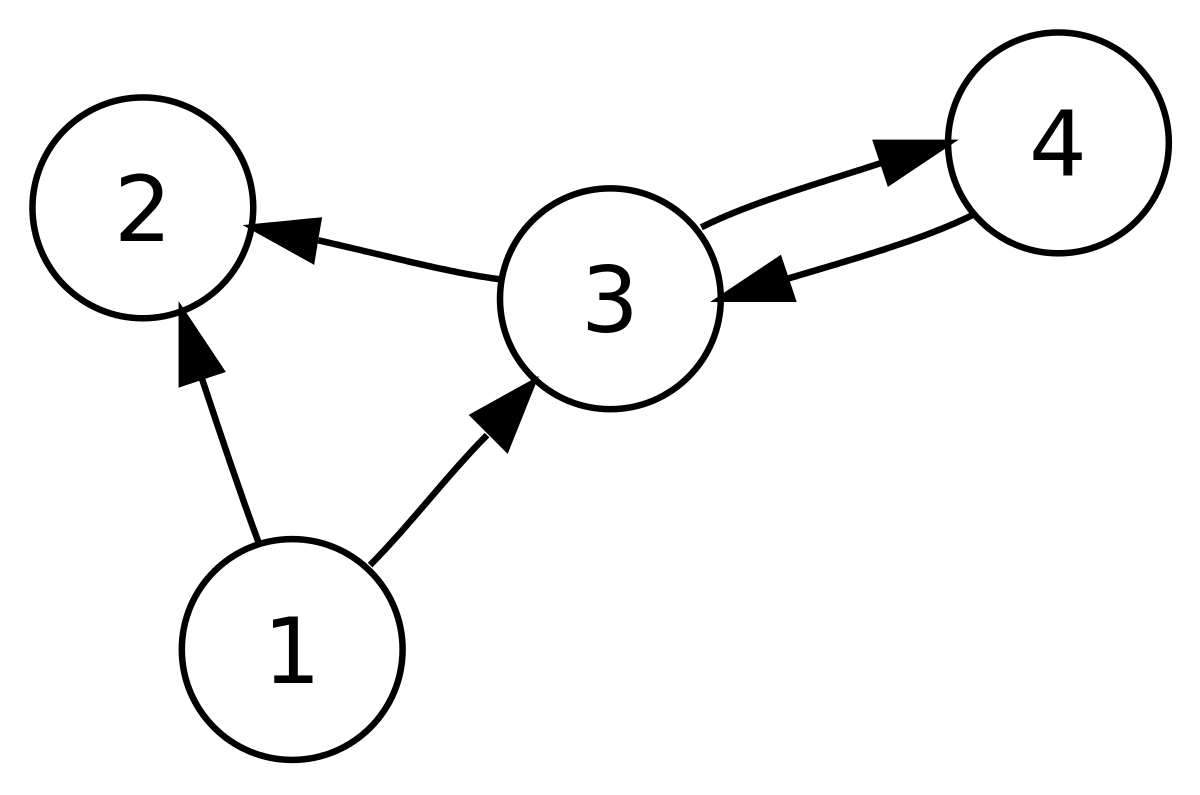
\includegraphics[scale=0.15,center]{./ressources/image/RepDiGraphe.png}
			\caption[Exemple de représentation graphique d'un digraphe.]{Exemple de représentation graphique d'un digraphe.}
			\label{grapheOr}
			\end{figure}
			
		
		\subsection{Quelques Propriétés:} %%% Arevoire 
			\begin{itemize}[label=$\circ$]
			\item\textbf{Ordre d'un digraphe:}
			est le nombre de sommets n = Card(V) \citep{DUT}.
			
			\item\textbf{taille d'un digraphe:} est le nombre d’arcs m = Card(A) \citep{DUT}.
			
			\item\textbf{Degré dans un digraphe:}
			Le degré d'un sommet $v_{i}$ $\in$ V dans un digraphe G=(V , E) est donnée par la formule :
			\begin{center}
				d($v_{i}$) = $d^+(v_{i}$) + $d^-(v_{i}$\\
			\end{center}			 
			 où $d^+(v_{i}$) est le nombre d'arcs sortants au sommet $v_{i}$ et est appelé degré extérieure et $d^-(v_{i}$) représente le nombre d'arcs incidents et est appelé degré intérieur \citep{muller}.
			 
			 \item\textbf{Voisinage dans un digraphe:}
			 Le voisinage d'un sommet $v_{i}$ $\in$ V, noté V($v_{i}$), dans un digraphe G = (V , E) est:
			 	\begin{center}
				V($v_{i}$) = succ($v_{i}$) $\bigcup$ pred($v_{i}$),
				\end{center}
				
				où succ($v_{i}$) est l'ensemble des successeurs de $v_{i}$ et pred($v_{i}$) est l'ensemble de ses prédécesseurs \citep{bac}, i.e le voisinage de $v_{i}$ est l'ensemble des sommets qui lui sont adjacents.
			
			\end{itemize}
			
		
	\section{Notion de Connexité}
	
	Les structures de graphes sont généralement exploitables à travers leurs interrogation qui permet de fournir des réponses aux problèmes modélisés. L'un des informations les plus importantes dans un graphe est la notion des relations (indirectes ou indirecte) entre deux nœuds ou plus formellement la connexité dans un graphe. Dans cette partie nous allons définir les concepts relatives à cette notion.
	
	\begin{itemize} [label = $\bullet$]
		
			 
			 \item \textbf{Chemin (resp. Chaine):}
			est une liste de sommets S= $(v_{0},v_{1},v_{2},...,v_{k})$ telle qu’il existe un arc (resp. une arête) entre chaque couple de sommets successifs.
			 
			 
			  \item \textbf{Cycle (resp. Circuit):} 
			 est un chemin (resp. chaine) dont le premier et le dernier sommet sont identiques \citep{DUT}.
			 
			 		\item \textbf{Graphe connexe:}
			Un graphe non orienté (resp. orienté) est dit connexe (resp. fortement connexe) si pour tout pair de sommets ($v_{i}$, $v_{j}$) il existe un chemin S les reliant \citep{muller}.
			 
		\end{itemize}
	
	
	
	\section{Graphe partiel et sous-graphe:}
    		
	La quantité de données disponible aujourd'hui et sa croissance de manière exponentielle ont favorisé la décomposition des graphes en des entités plus petites afin de garantir une facilité de compréhension et d'analyse dans le but d'extraire l'information la plus pertinente. Dans cette partie, nous allons définir de manière plus formelle ce que ces entités sont, ainsi que leurs types.
	
		
		
		
		\subsection{Définitions:}
		Soient G = (V , E), $G' = (V' , E')$ et $G'' = (V'' , E'')$ trois graphes.
		\begin{itemize}[label=$\circ$]
		
			\item Le graphe $G'$ est appelé \textbf{graphe partiel} de G si : $V' = V\ et\ E' \subset$ E \citep{DUT}. En d'autres termes, un graphe partiel est obtenu en supprimant une ou plusieurs arêtes de G.
				

			\item Le graphe $G''$ est dit \textbf{sous-graphe} de G si: $V''\subset V$ et 
			 $E''\subset E \cap (V'' x V'')$ \citep{bac}, i.e, un sous-graphe est obtenu en enlevant un ou plusieurs nœuds du graphe initial ainsi que les arêtes dont ils représentent l'une des deux extrémités.
			 
		\end{itemize}
		
		\subsection{Quelques Types de sous graphes:}
		
		\begin{itemize} [label = $\bullet$]
		
		
			\item \textbf{Une Clique :} est un sous-graphe complet de G \citep{bac}.
			
			\item \textbf{Biparti :} G' est un sous-graphe biparti si il existe une partition de V' en deux sous ensembles notés $V_{1}$ et $V_{2}$, i.e V' = $V_{1} \cup V_{2}$ et $V_{1}$ $\cap$ $V_{2}$ = $\phi$, tel que E' = $V_{1}$ x $V_{2}$ \citep{bac}.
			
			\item \textbf{Étoile :}
			 est un cas particulier de sous-graphe biparti où $V_{1}$ est un ensemble contenant le sommet central (dit \textit{hub}) uniquement et $V_{2}$ contient le reste des nœuds  (dits \textit{spokes})\citep{koutra2015summarizing} .
			 
		
			 
		\end{itemize}		
	
	\section{Quelques types de graphe}
		 %% classifier selon le type du graphe en entree
	Avec les avancées technologiques au fil du temps, plusieurs types de graphes ont connus le jours. En effet, La complexité et la variété des problèmes scientifiques existants modélisés par ces derniers ont poussé les chercheurs à adapter leurs structure selon le problème auquel ils font face. Durant cette section nous allons définir les principaux types existants.
	
		\begin{itemize}[label=$\circ$]
		
			\item \textbf{Graphe Complet:} Un graphe G = (V , E) est un graphe complet si tous les sommets $v_{i}$ $\in$ V sont adjacents \citep{Pres}. Il est souvent noté $K_{n}$ où n = card(V) \citep{DUT}.
				
			
			\item \textbf{Graphe étiqueté et graphe pondéré:}
			 Un graphe étiqueté G = (V , E , W) est un graphe, qui peut être orienté ou non orienté, dont chacune des arêtes $e_{i}$ $\in$ E est doté d'une étiquette $w_{i}$. Si de plus, $w_{i}$ est un nombre alors G est dit graphe pondéré (valué) \citep{DUT}.
		
			\item \textbf{Graphe simple et graphe multiple:}
			Un graphe G = (V , E) est dit simple si il ne contient pas de boucles et toute paire de sommets est reliée par au plus une arête. Dans le cas contraire, G est dit multiple \citep{IUTLyonInformatique}.
			
		
		\end{itemize}
			
	
	
    		
    	\section{Représentation Structurelle d'un graphe}	
		\input{./Chapitres/TheorieDesGraphes/structRep.tex}
	
	\section{Les domaines d'application}
		  La diversité des domaines faisant appel à la modélisation par des graphes ne cesse d'augmenter, allant des réseaux sociaux aux réseaux électriques et réseaux biologiques et arrivant jusqu'aux World Wide Web. Dans cette partie nous allons décrire trois domaines d'application les plus répandus des graphes.
	
		\subsection{Graphes des réseaux sociaux:}
		Les réseaux sociaux représentent un lieu d'échange et de rencontre entre individus (entités) et dont l'utilisation est devenue de nos jours une nécessité.  
		Pour représenter les interactions entre ces individus, nous avons généralement besoin de faire recours aux graphes où les sommets sont des individus ou des entités et les interactions entre eux sont représenté par des liens. 
		Vue la diversité des interactions sociales, la modélisation de ces réseaux  nécessite différents types de graphes: graphes non orientés pour pour les réseaux sociaux avec des relations non
orientées, graphes orientés pour représenter des relations non symétriques
comme c'est la cas dans les réseaux de confiance, graphes pondérés pour les réseaux sociaux qui contiennent différents niveaux d'intensités dans les relations, ... etc \citep{lemmouchi2012etude}.
		
		\subsection{Graphes en Bioinformatique:}
		
		La bio-informatique est un domaine qui se trouve à l'intersection des deux grands domaines celui de l'informatique et celui de la biologie. Elle a pour but d'exploiter la puissance de calcule des équipements informatiques pour effectuer des traitements sur des données moléculaires massives \citep{pellegrini2004protein}.
		
		Elle est largement utilisée pour l’analyse des séquences d’ADN et des protéines à travers leurs modélisation sous forme de graphe. A titre d'exemple, les graphes non orientés multiples sont un outil modélisation des réseaux d’interaction protéine-protéine \citep{pellegrini2004protein}, 
		le but dans ce cas est donc l'étude du fonctionnement des protéines par rapport à d'autre.
		
		\subsection{Le Graphe du web:}
		 Le graphe du Web est un graphe orienté dont les sommets sont les pages du web et les arêtes modélise l'existence d'un lien hypertexte dans une page vers une autre \citep{brisaboa2009k}. Il représente l'un des graphes les plus volumineux: en juillet 2000 déja, on estimait qu’il contenait environ 2,1 milliards de sommets et 15 milliards d’arêtes avec 7,3 millions de pages ajoutées chaque jour \citep{guillaume2002web}. De ce fait, ce graphe a toujours attiré l'attention des chercheurs. En effet, l'étude de ses caractéristiques a donné naissance à plusieurs algorithmes intéressants, notamment l'algorithme PageRank de classement des pages web qui se trouve derrière le moteur de recherche le plus connu de nos jours : Google.	
		
	
	
			
	\section{Conclusion}
Dans ce chapitre nous avons présenté les notions et les concepts généraux qui touchent à la théorie des graphes : définitions des graphes, leurs principales propriétés, leurs représentations ainsi que leurs domaines d'application.\\
Le point important qu'on a pu tirer de cette partie est que les graphes sont devenus un moyen crucial et indispensable dans la modélisation des problèmes dans plusieurs domaines. Cependant ils deviennent de plus en plus complexes et volumineux avec la grande quantité de données disponible de nos jours. De ce fait, leur stockage, visualisation et traitement sont devenus difficile. La compression de graphe est naît comme solution à ce problème. Dans le chapitre suivant nous allons présenter la compression de graphes, son rôle et ses différentes méthodes.  
	
	